\documentclass[aps,preprint,nofootinbib,floatfix]{revtex4-1}

%\usepackage{cite}
\usepackage[pdftex]{graphicx}
\graphicspath{{./figures/}}
%\graphicspath{{./}}
\usepackage{amsmath,amssymb,amsfonts,amsthm,amscd,bm}
\usepackage{bbm}
\usepackage{algorithm}
\usepackage{algorithmic}
%\usepackage{epstopdf}
%\usepackage{fixltx2e}
%\usepackage{stfloats}

\hyphenation{op-tical net-works semi-conduc-tor}

\newtheorem{theorem}{Theorem}
\newtheorem{definition}[theorem]{Definition}
\newtheorem{assumption}[theorem]{Assumption}
\newtheorem{lemma}[theorem]{Lemma}
\newtheorem{corollary}[theorem]{Corollary}
\newtheorem{proposition}[theorem]{Proposition}
\newtheorem{conjecture}[theorem]{Conjecture}
\newtheorem{remark}[theorem]{Remark}
\newtheorem{example}{Example}

%% our definitions %%%%%%%%%%%%%%%%%%%%%%%%%%%%%%%%%%%%%%%%%%%%%%%%%%%%%%%%%%%%
\DeclareMathOperator{\aff}{aff}
\DeclareMathOperator{\st}{s.t.}
\DeclareMathOperator{\LC}{LC}
\DeclareMathOperator{\affnot}{aff_0}
\DeclareMathOperator{\conv}{conv}
\DeclareMathOperator{\relint}{relint}
\DeclareMathOperator{\vol}{vol}
\DeclareMathOperator{\range}{range}
\DeclareMathOperator{\image}{im}
\DeclareMathOperator{\nullspace}{null}
\DeclareMathOperator{\area}{area}
\DeclareMathOperator{\vspan}{span}
\DeclareMathOperator{\id}{Id}
\DeclareMathOperator{\cond}{cond}
\DeclareMathOperator{\prox}{prox}
\DeclareMathOperator*{\argmax}{arg\,max}
\DeclareMathOperator*{\argmin}{arg\,min}
\DeclareMathOperator*{\minimize}{minimize}
\DeclareMathOperator{\diag}{diag}
\DeclareMathOperator{\Tr}{Tr}

\graphicspath{{figs/}}

\begin{document}

\title{Notes about Statistics, Clustering, Graphs, \ldots}

\author{Guilherme Fran\c ca}

\begin{abstract}
In this document we collect notes about our experiments and theories
so we can discuss together with the group in an organized way.
\end{abstract}

\maketitle


%%%%%%%%%%%%%%%%%%%%%%%%%%%%%%%%%%%%%%%%%%%%%%%%%%%%%%%%%%%%%%%%%%%%%%%%%%%%%%%
\section{Experiments using Energy Statistics and One-Dimensional 
Random Projections (Gui 04-01-2017)}

Given data $X=\{ x_i \}_{i=1}^{n}$, where $x_i \in \mathbb{R}^{D}$, 
and the number of clusters $k$, we perform the following experiments:
\begin{enumerate}
\item Run $k$-means++ 
on the original data. This is the column named 
``$k$-means'' in the following tables.
\item Use PCA to 
project the data in the first principal component, 
$Y=\{ y_i \}_{i=1}^n$ where $y_i = u_{1}\cdot x_i \in \mathbb{R}$, then
apply $k$-means++ in this $1$-dimensional space. This is the column named
``PCA'' in the following tables.
\item We randomly project the data in one dimension by picking a vector
$w$ such that $w_i \sim \mathcal{N}(0,1)$ and normalize it $\| w \|=1$.
Thus $Y = \{y_i\}_{i=1}^n $ where $y_i = w\cdot x_i \in \mathbb{R}$. 
We apply $k$-means++ in this randomly projected
$1$-dimensional space. We do this several times and pick the best answer,i.e.
the one which has minumim objective function in the \emph{original} space,
since it is cheap to compute this objective function.
This is the column named ``$k$-random'' in the following tables.
\item We use random projections as in the previous item, but use the $T$-test
from energy statistics. In $1D$ we can compute the energy distance in an
efficient manner if we sort the data $Y$. This is accomplished in
$O(n\log n)$. This is the column called
``$\mathcal{E}$-random'' in the following tables. We pick the best answer
by computing the largest $T$, in the one-dimensional space.
\end{enumerate}

The evaluation of the clustering procedure 
will be based on the true labels by the following quantity, called
accuracy:
\begin{equation}
\label{eq:accuracy}
a(z,\hat{z}) = 
\dfrac{1}{n}\sum_{i=1}^{n} \mathbbm{1}\left(z_i = \pi(\hat{z}_i) \right)
\end{equation}
where $z$ is an $n$-dimensional vector containing the true labels, entry
$z_i$ corresponds to point $x_i$, and $\hat{z}$ is the estimated labels
through the clustering procedure. $\pi$ is a permutation of the labels.
Thus the above formula gives $a=1$ if all points were correctly classified and
$a=0$ if all points were wrongly classified. In a two class problem with
the same number of points, $a=1/2$ corresponds to picking the points in each
cluster at random. 
This quantity $a$ is the number shown in the following tables.


In the first experiment shown in Fig.~\ref{fig:2d_gauss_sep} we choose
two well separated gaussians in $2D$. All of these procedures give good
results.

\begin{figure}
\begin{minipage}{.49\textwidth}
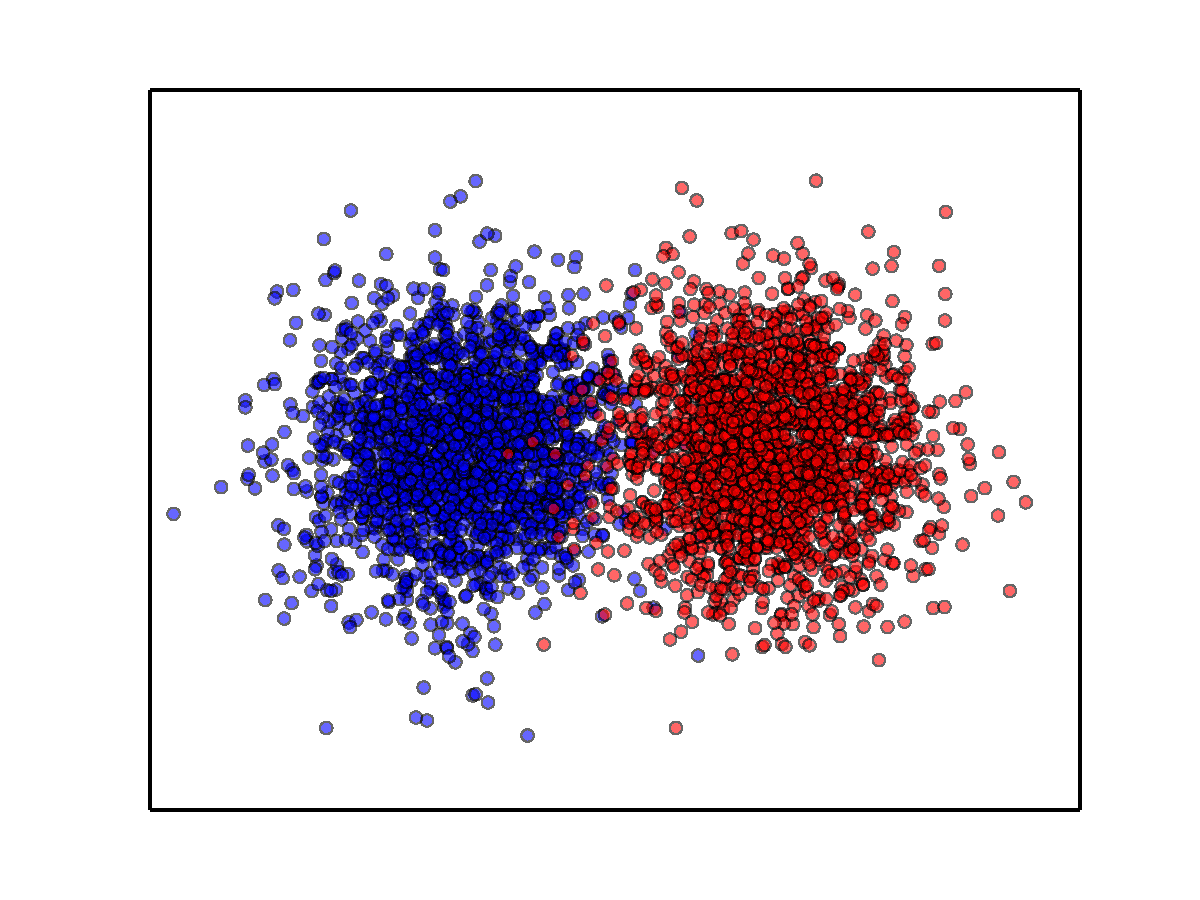
\includegraphics[scale=.45]{2d_gauss_separate.pdf}
\end{minipage}
\begin{minipage}{.49\textwidth}
\begin{tabular}{ l  l  l l}
\hline
$k$-means~ & PCA~~~ & $k$-random~ & $\mathcal{E}$-random \\
\hline
0.97775 &
0.97825 & 
0.79925 &
0.977 \\
0.975 &
0.975 &
0.7305 &
0.976 \\
0.9765 &
0.9765 &
0.9655 &
0.9605 \\
%
\hline
\end{tabular}
\end{minipage}
\caption{\label{fig:2d_gauss_sep}
We have $x \sim \tfrac{1}{2}\left( \mathcal{N}(\mu_1, I) +
\mathcal{N}(\mu_2, I)\right)$ where $\mu_1 = (0,0)^T$ and $\mu_2=(4,0)^T$,
and $1000$ points on each cluster. We run the experiment three times.
We choose only $20$ random projections.
}
\end{figure}

\begin{figure}
\begin{minipage}{.49\textwidth}
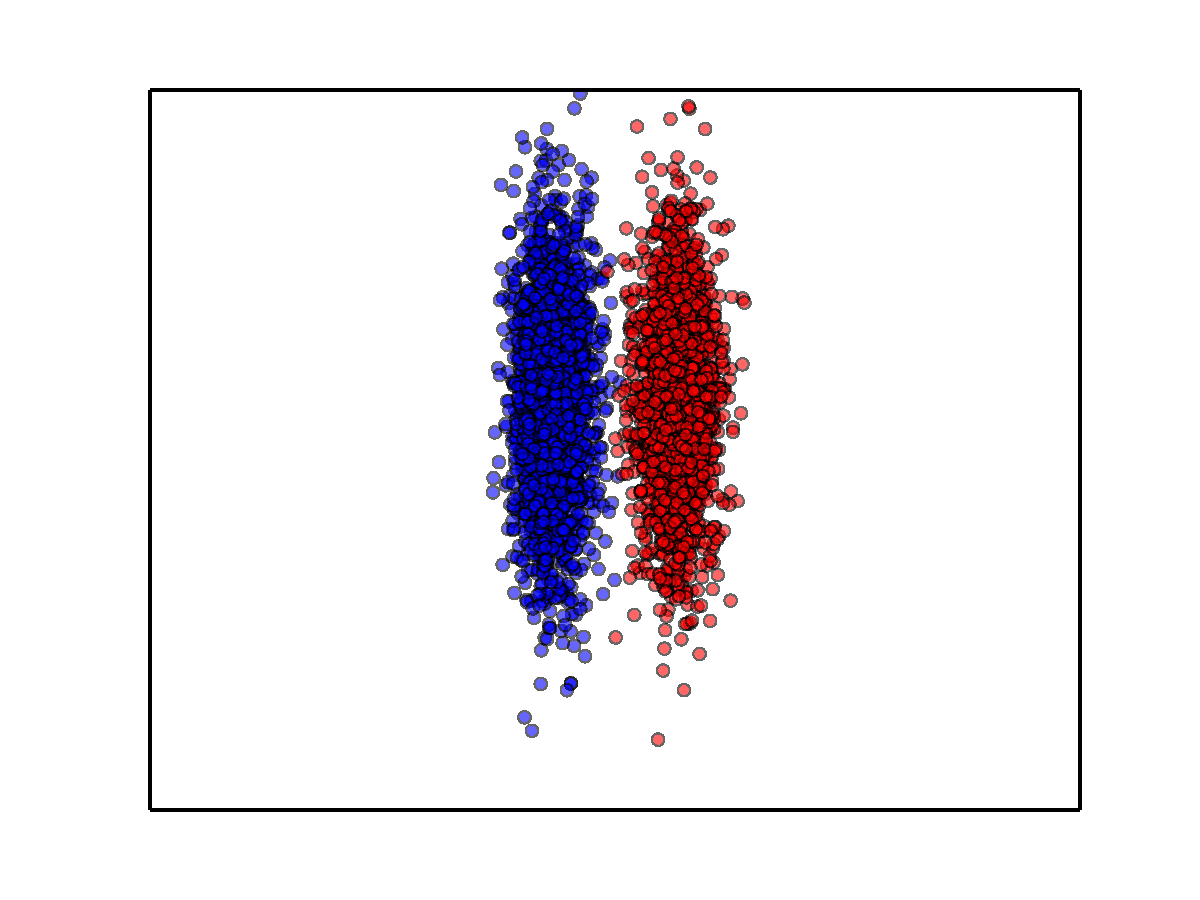
\includegraphics[scale=.45]{2d_cigar.pdf}
\end{minipage}
\begin{minipage}{.49\textwidth}
\begin{tabular}{ l l l l}
\hline
$k$-means~ & PCA~~~ & $k$-random~ & $\mathcal{E}$-random \\
\hline
0.51325 &
0.506 &
0.70325 &
0.977 \\
0.52175 &
0.5105 &
0.54725 &
0.7295 \\
0.53325 &
0.53175 &
0.9785 &
0.998 \\
%
\hline
\end{tabular}
\end{minipage}
\caption{\label{fig:cigar}
We have $x \sim \tfrac{1}{2}\left( \mathcal{N}(\mu_1, \Sigma) +
\mathcal{N}(\mu_2, \Sigma)\right)$ where $\mu_1 = (0,0)^T$, $\mu_2=(6,0)^T$,
and $\Sigma = \left( \begin{smallmatrix} 1 & 0 \\ 0 & 20 \end{smallmatrix}
\right)$,
and $2000$ points on each cluster. We run the experiment three times.
We use $30$ random projections.
}
\end{figure}


\begin{figure}
\begin{minipage}{.49\textwidth}
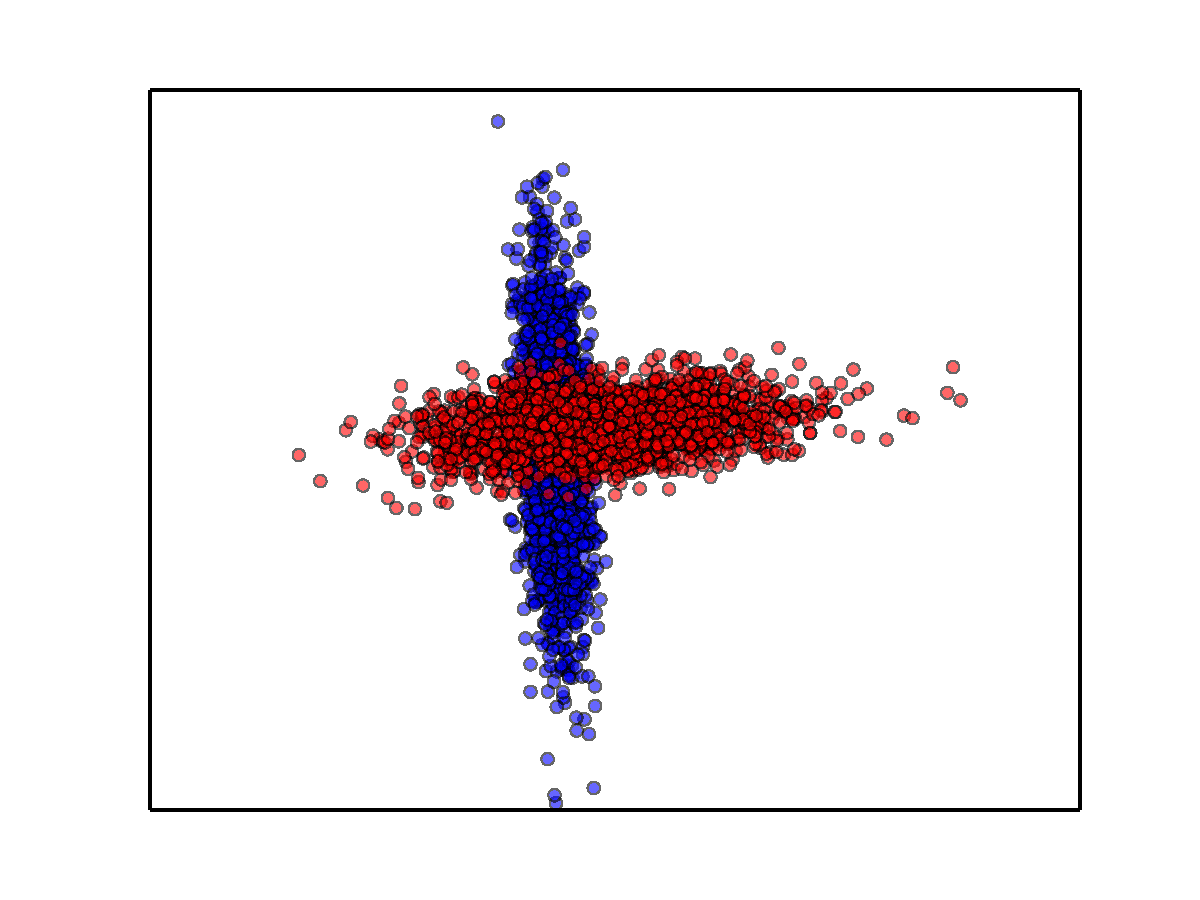
\includegraphics[scale=.45]{2d_weird1.pdf}
\end{minipage}
\begin{minipage}{.49\textwidth}
\begin{tabular}{ l l l l}
\hline
$k$-means~ & PCA~~~ & $k$-random~ & $\mathcal{E}$-random \\
\hline
0.71275 &
0.68675 &
0.51275 &
0.6505 \\
0.7235 & 
0.6645 & 
0.6095 & 
0.641 \\
0.72575 &
0.68475 &
0.60975 &
0.509 \\
\hline
\end{tabular}
\end{minipage}
\caption{\label{fig:weird1}
We have $x \sim \tfrac{1}{2}\left( \mathcal{N}(\mu_1, \Sigma_1) +
\mathcal{N}(\mu_2, \Sigma_2)\right)$ where $\mu_1 = (0,0)^T$, $\mu_2=(2,1)^T$,
$\Sigma_1 = \left( \begin{smallmatrix} 0.5 & -0.8 \\ -0.8 & 15 
\end{smallmatrix}
\right)$,
$\Sigma_2 = \left( \begin{smallmatrix} 15 & 1 \\ 1 & 1 \end{smallmatrix}
\right)$,
and $2000$ points on each cluster. We run the experiment three times,
with 30 random projections.
}
\end{figure}


In the experiment of Fig.~\ref{fig:highd} we increase the number of
dimensions of the gaussian distributions. Both $k$-means and PCA perform well
if the dimension is not too high, while $1D$ random projections provide
poor results. This is also expected since randomly projecting high dimensional
data in a very low dimensional space practically destroy any information
about the original distribution.

\begin{figure}
\begin{minipage}{.49\textwidth}
\centering
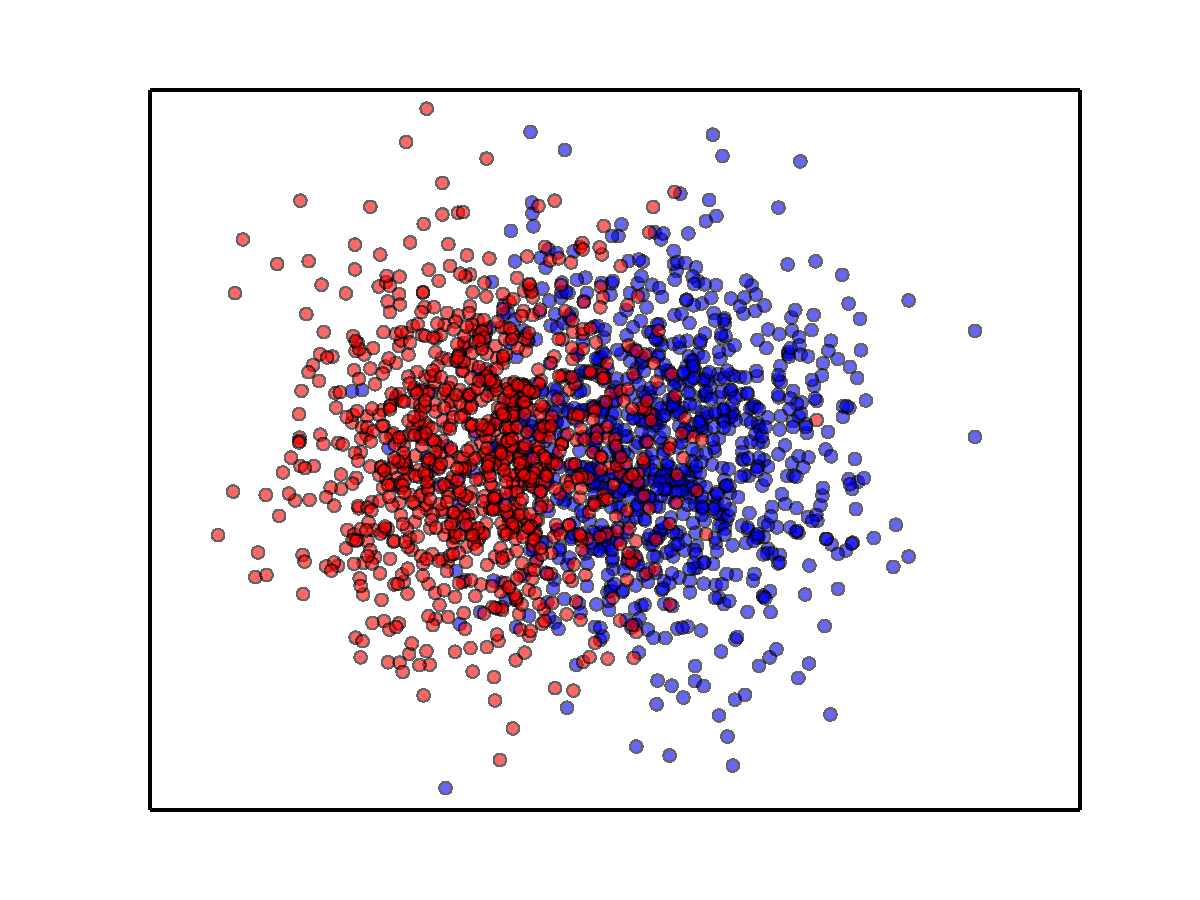
\includegraphics[scale=.45]{30d_gauss.pdf}
\end{minipage}
\begin{minipage}{.5\textwidth}
\renewcommand*{\arraystretch}{.3}
\begin{tabular}{l l l l l}
\hline
$D$ & $k$-means & PCA & $k$-random & $\mathcal{E}$-random \\
\hline
%
5 & 0.928000 & 0.928000 & 0.689500 & 0.859000 \\
10 & 0.935500 & 0.935500 & 0.551000 & 0.890000 \\
15 & 0.929000 & 0.930000 & 0.580500 & 0.839000 \\
20 & 0.938000 & 0.940000 & 0.647000 & 0.741000 \\
25 & 0.937500 & 0.936500 & 0.576500 & 0.801000 \\
30 & 0.939000 & 0.938500 & 0.545000 & 0.565000 \\
50 & 0.933500 & 0.930000 & 0.505500 & 0.701000 \\
100 & 0.928500 & 0.932000 & 0.624500 & 0.565000 \\
200 & 0.935000 & 0.935000 & 0.502000 & 0.528000 \\
300 & 0.922500 & 0.924500 & 0.508500 & 0.527000 \\
500 & 0.916500 & 0.923500 & 0.509000 & 0.513000 \\
1000 & 0.881000 & 0.889500 & 0.503000 & 0.501000 \\
2000 & 0.615000 & 0.867000 & 0.509500 & 0.505000 \\
5000 & 0.534500 & 0.780000 & 0.514000 & 0.511000 \\
%
\hline
\end{tabular}
\end{minipage}
\caption{\label{fig:highd}
High dimensions.
We have $x \sim \tfrac{1}{2}\left( \mathcal{N}(\mu_1, I_D) +
\mathcal{N}(\mu_2, I_D)\right)$ where $\mu_1 = (0,0,\dotsc,0)^T$,
$\mu_2=(3,0,\dots,0)^T$,
and $1000$ points on each cluster. We do 100 random projections.
We show the two principal components
of the data in the plot above.
}
\end{figure}


\begin{figure}
\begin{minipage}{.49\textwidth}
\centering
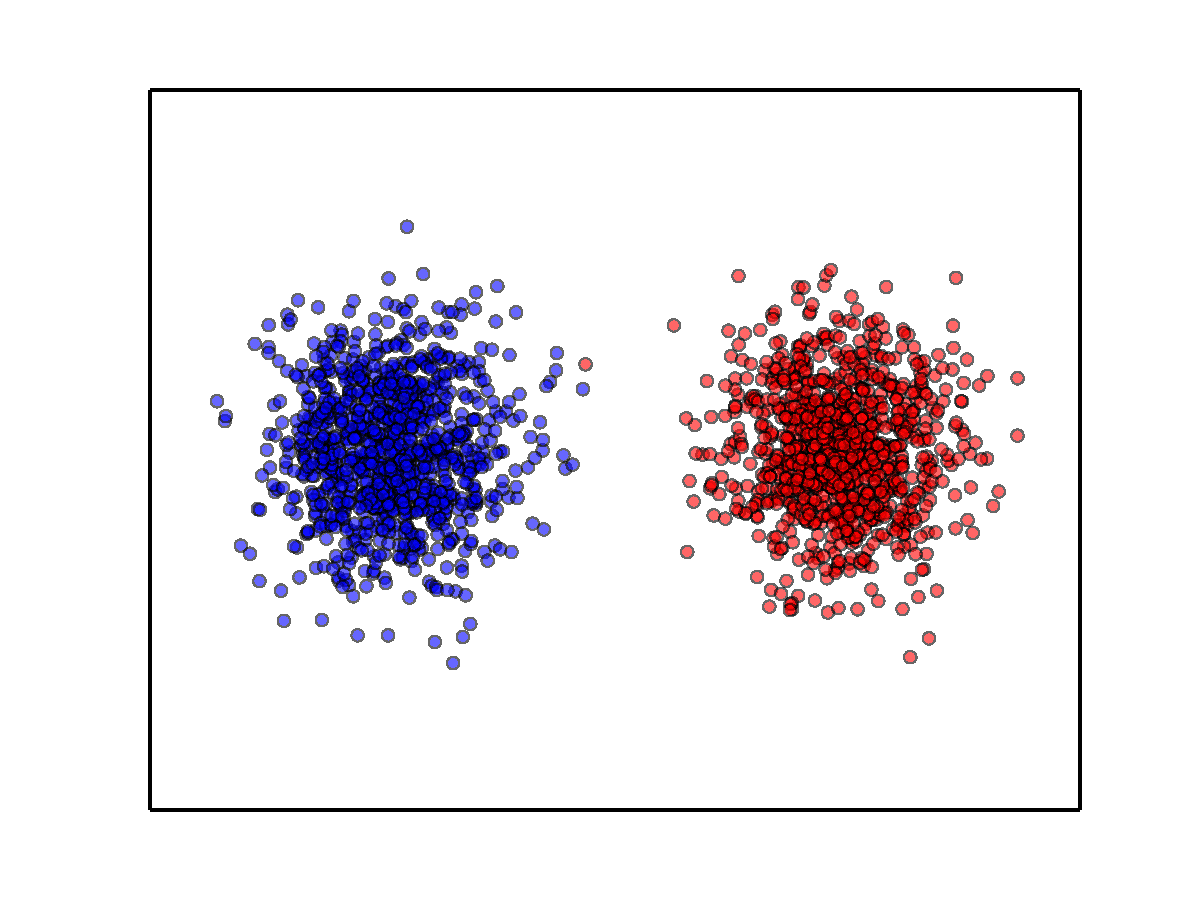
\includegraphics[scale=.45]{30d_more_signal_guass.pdf}
\end{minipage}
\begin{minipage}{.5\textwidth}
\renewcommand*{\arraystretch}{.3}
\begin{tabular}{l l l l l}
\hline
$D$ & $k$-means & PCA & $k$-random & $\mathcal{E}$-random \\
\hline
%
5 & 0.963000 & 0.963000 & 0.615000 & 0.921000 \\
10 & 0.985500 & 0.985000 & 0.758000 & 0.957000 \\
15 & 0.998000 & 0.998000 & 0.537500 & 0.919000 \\
20 & 0.998500 & 0.998500 & 0.505500 & 0.889000 \\
25 & 1.000000 & 1.000000 & 0.530000 & 0.968000 \\
30 & 1.000000 & 1.000000 & 0.733500 & 0.978000 \\
50 & 1.000000 & 1.000000 & 0.640000 & 0.957000 \\
100 & 1.000000 & 1.000000 & 0.887500 & 0.972000 \\
200 & 1.000000 & 1.000000 & 0.708500 & 0.964000 \\
300 & 1.000000 & 1.000000 & 0.549000 & 0.967000 \\
500 & 1.000000 & 1.000000 & 0.653000 & 0.968000 \\
1000 & 1.000000 & 1.000000 & 0.604500 & 0.983000 \\
2000 & 1.000000 & 1.000000 & 0.535000 & 0.967000 \\
5000 & 1.000000 & 1.000000 & 0.727500 & 0.949000 \\
%
\hline
\end{tabular}
\end{minipage}
\caption{\label{fig:highd}
High dimensions.
We have $x \sim \tfrac{1}{2}\left( \mathcal{N}(\mu_1, I_D) +
\mathcal{N}(\mu_2, I_D)\right)$ where 
$\mu_1 = (1,0,1,\dotsc,0,1)^T$,
$\mu_2 = (-1,0,-1,\dotsc,0,-1)^T$, i.e. the even dimensions are
shifted at $+1$ and $-1$, respectivelly.
We have $1000$ points on each cluster. We do 100 random projections.
We show the two principal components
of the data in the plot above. When we have more signal we can see that
random projections with $\mathcal{E}$ is much superior to random projections
and $k$-means++.
}
\end{figure}


\subsection{Conclusions}
If we have enough signal, even in high dimensions random projections with
energy statistics seems like a good thing. I believe that at least for
a initialization procedure this can be usefull. It will be interesting to
have a benchmark of how many random projections we need. Too many is expensive,
however, if this is an initialization procedure, it will be required only
once. Maybe we can compare just $\mathcal{E}$-random with the initialization
provided by $k$-means++.


%%%%%%%%%%%%%%%%%%%%%%%%%%%%%%%%%%%%%%%%%%%%%%%%%%%%%%%%%%%%%%%%%%%%%%%%%%%%%%%
\section{Energy Statistics Based Clustering (Gui 04-05-2017)}


We show some experiments regarding our method for clustering using energy
statistics. We have a QCQP approximation to the original problem, and we solve
this QCQP through a relaxation, thus there are two approximations going on
here. We solve this through a kernel approach. The function has a maximum, but
it is really sensitive to initialization, since apparently there are lots of
local minima. We use energy statistics in $1D$ with random projections for
initialization. This seems to provide a better initialization than pure random
or even k-means.

\begin{figure}
\begin{minipage}{.49\textwidth}
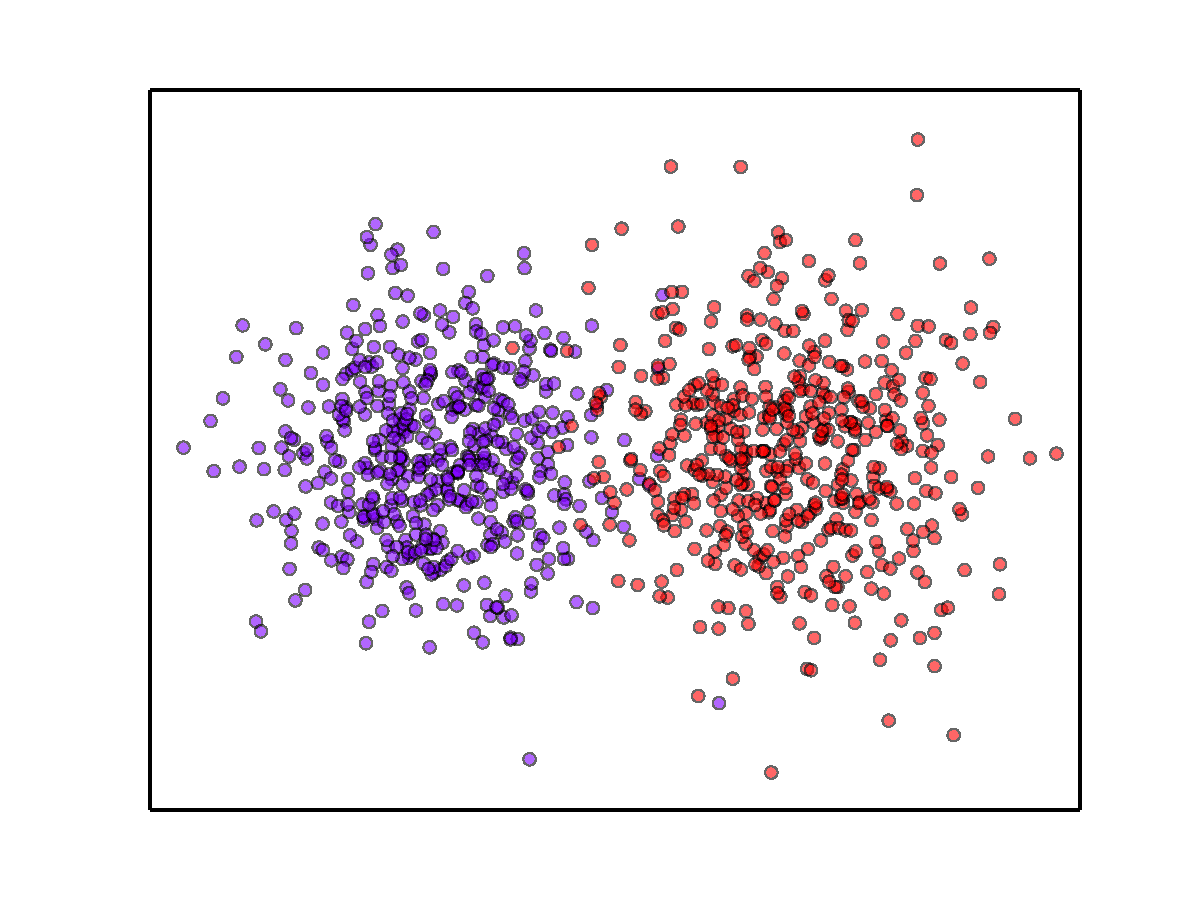
\includegraphics[scale=.45]{two_gaussians_separated.pdf}
\end{minipage}
\begin{minipage}{.49\textwidth}
\begin{tabular}{ l l l l l}
\hline
Ker/$\mathcal{E}$ & Ker/Gauss & Ker/Poly & GMM~~ & $k$-means \\
\hline
0.97 &
0.965 &
0.863 &
0.969 & 
0.971 \\
0.98 &
0.98 &
0.878 &
0.982 &
0.98 \\
0.982 &
0.982 &
0.877 &
0.983 &
0.983 \\
\hline
\end{tabular}
\end{minipage}
\caption{\label{fig:weird1}
We have $x \sim \tfrac{1}{2}\left( \mathcal{N}(\mu_1, \Sigma_1) +
\mathcal{N}(\mu_2, \Sigma_2)\right)$ where $\mu_1 = (0,0)^T$, $\mu_2=(4,0)^T$,
$\Sigma_1 = \Sigma_2 = I$,
and $500$ points on each cluster. We run the experiment three times,
with 20 random projections as initialization.
}
\end{figure}

\begin{figure}
\begin{minipage}{.49\textwidth}
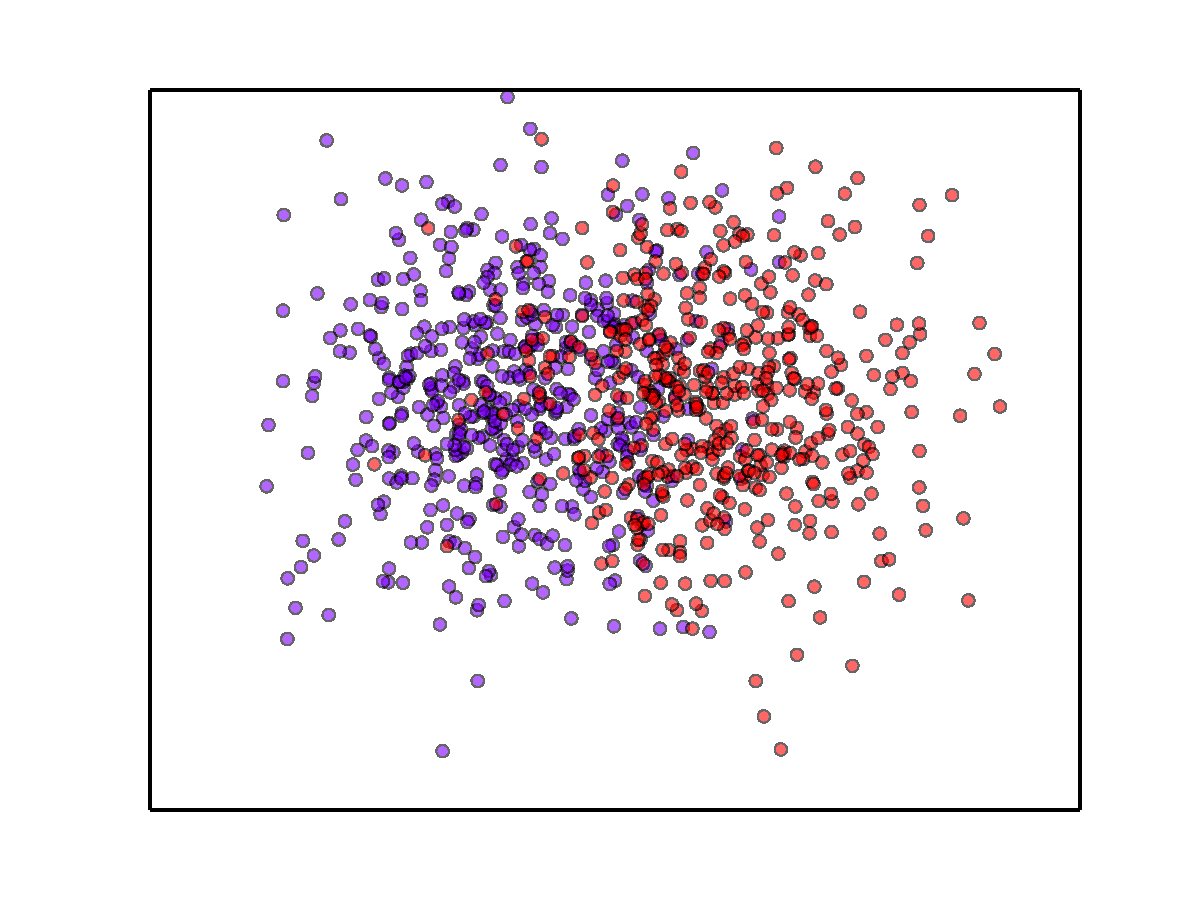
\includegraphics[scale=.45]{two_gaussians_closer.pdf}
\end{minipage}
\begin{minipage}{.49\textwidth}
\begin{tabular}{ l l l l l}
\hline
Ker/$\mathcal{E}$ & Ker/Gauss & Ker/Poly & GMM~~ & $k$-means \\
\hline
0.844 &
0.829 &
0.688 &
0.841 &
0.843 \\
0.834 &
0.836 &
0.695 &
0.835 &
0.834 \\
0.843 &
0.813 &
0.68 &
0.805 &
0.841 \\
\hline
\end{tabular}
\end{minipage}
\caption{\label{fig:weird1}
We have $x \sim \tfrac{1}{2}\left( \mathcal{N}(\mu_1, \Sigma_1) +
\mathcal{N}(\mu_2, \Sigma_2)\right)$ where $\mu_1 = (0,0)^T$, $\mu_2=(2,0)^T$,
$\Sigma_1 = \Sigma_2 = I$,
and $500$ points on each cluster. We run the experiment three times,
with 20 random projections as initialization.
}
\end{figure}

\begin{figure}
\begin{minipage}{.49\textwidth}
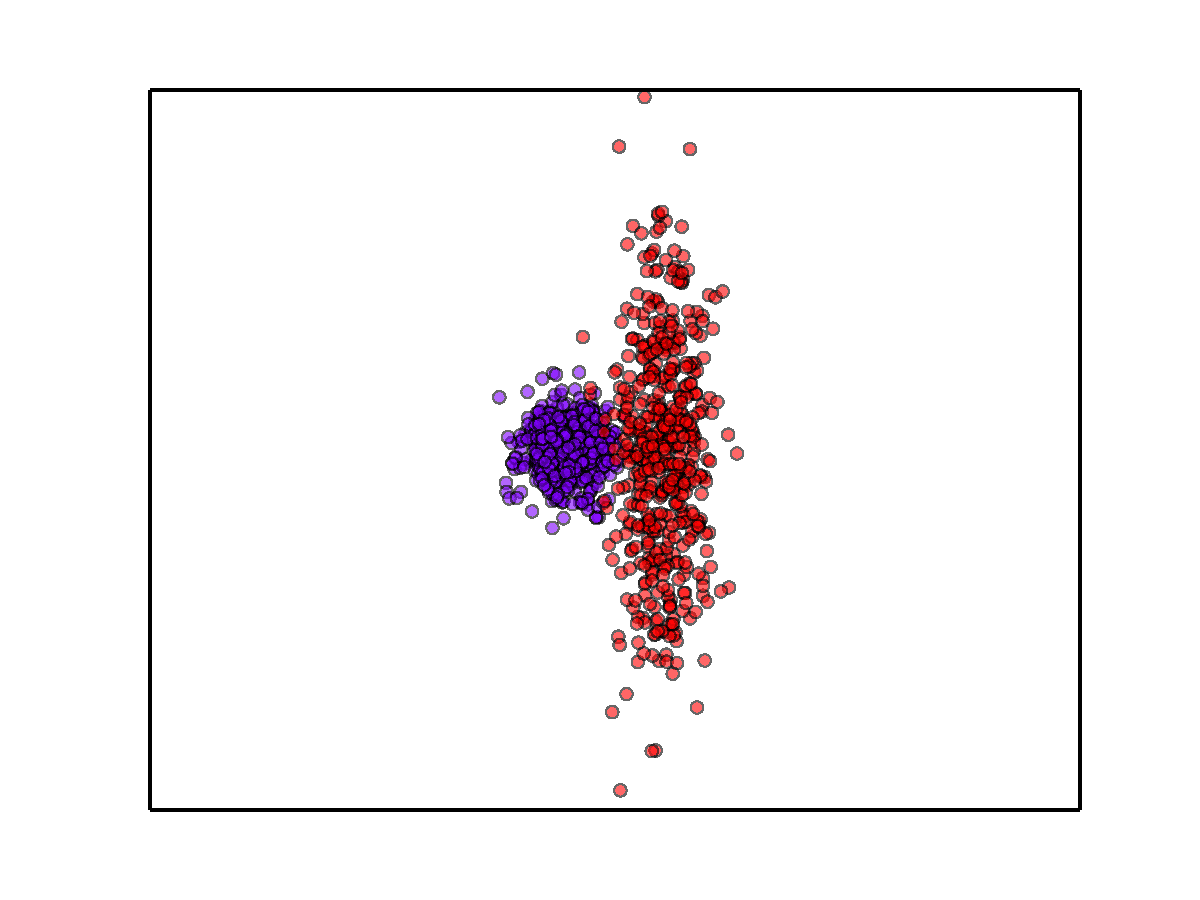
\includegraphics[scale=.45]{blob_cigar.pdf}
\end{minipage}
\begin{minipage}{.49\textwidth}
\begin{tabular}{ l l l l l}
\hline
Ker/$\mathcal{E}$ & Ker/Gauss & Ker/Poly & GMM~~ & $k$-means \\
\hline
0.988 &
0.807 &
0.603 &
0.988 & 
0.7 \\
0.981 & 
0.831 &
0.603 &
0.983 & 
0.698 \\
0.731 & 
0.789 &
0.626 & 
0.986 &
0.717 \\
\\
\hline
\end{tabular}
\end{minipage}
\caption{\label{fig:weird1}
We have $x \sim \tfrac{1}{2}\left( \mathcal{N}(\mu_1, \Sigma_1) +
\mathcal{N}(\mu_2, \Sigma_2)\right)$ where $\mu_1 = (0,0)^T$, $\mu_2=(4,0)^T$,
$\Sigma_1 = I$, 
$\Sigma_2 = \left( \begin{smallmatrix} 
1 & 0 \\ 1 & 20
\end{smallmatrix}\right)$
and $500$ points on each cluster. We run the experiment three times,
with 20 random projections as initialization.
}
\end{figure}


\end{document}
